\documentclass[12pt]{beamer}
\beamertemplatenavigationsymbolsempty

\usetheme{Copenhagen}
\useoutertheme{infolines}

\usepackage[utf8]{inputenc}
\usepackage[ngerman]{babel}
\usepackage{graphicx}
\usepackage{subfigure}
\title[Task6]{Task 6 \\Auswertung MPGA\\Günstige und Ungünstige Parametrisierungen}
\institute{EvoTest}
\author{Alex, Yaroslav, Manuel}
\date{01.02.2017}

\begin{document}
\maketitle

\section{Vorgehen}
\frame{
\frametitle{Allgemeines Vorgehen}
Ziel: Vergleich verschiedener Parametrisierungen des Multi-Population Genetic Algorithms.
\begin{itemize}
	\item Kombination von Migrationsrate und Migrationsinterval
	\item Migrationsstrategien
\end{itemize}
}

\frame{
\frametitle{Allgemeines Vorgehen}
Vorgehen:
\begin{enumerate}
	\item Erschaffen einer Vergleichsbasis:\\
	MPGA ohne Migration laufen lassen $\rightarrow$ Simuliert mehrere einzelne Single Population Genetic 
	\item MPGA mit Migration und unterschiedlichen Konfigurationen laufen lassen
\end{enumerate}
}

\frame{
\frametitle{Allgemeines Vorgehen}
Rahmenbedingungen:
\begin{itemize}
	\item Anzahl Epochen: 1.000.\\
	Fitness-Werte stagnieren vor dieser Grenze.\\
	Ermittelt im Migrationsfreien Lauf.
	\item Populationsgröße: 8.\\
	Groß genug für ausreichende Diversität pro Population.\\
	Klein genug für angemessene Laufzeit.
	\item Fitnessfunktionen spiegeln Testfälle wider:\\
	Positioniert links und rechts des Parkplatzes.\\
	Orientiert nach oben, unten, links und rechts.
\end{itemize}
}

\frame{
\frametitle{Allgemeines Vorgehen}
Auswertung:
\begin{itemize}
	\item Vergleich der Entwicklung der durchschnittlichen Fitness-Werte der Populationen.
	\item Vergleich der generierten Testfälle.
\end{itemize}
}

\frame{
\frametitle{Migrationsfreier Durchlauf}
\begin{figure}
\centering
	\subfigure[Mittlere Fitness\label{fig:plain_fit}]{
		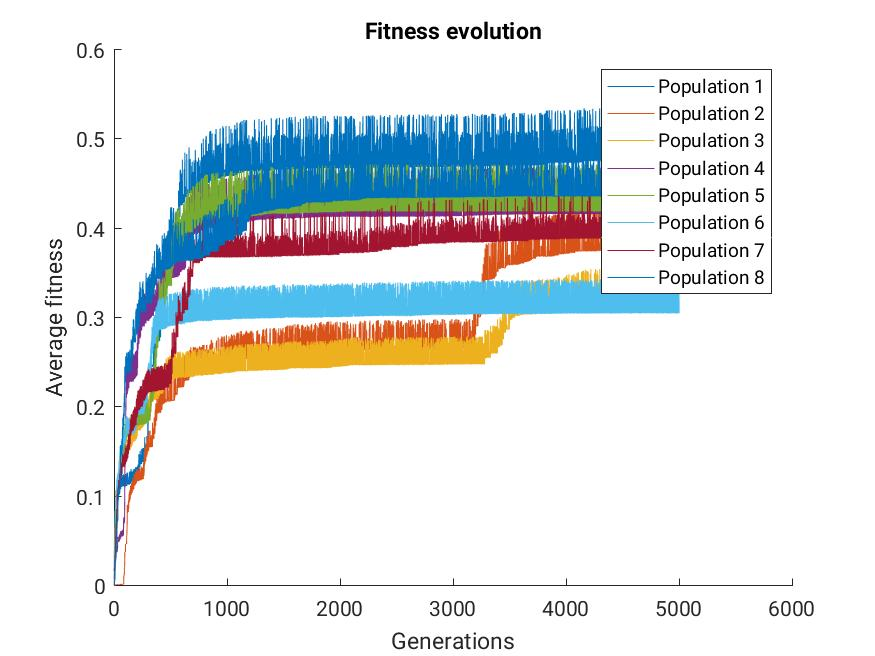
\includegraphics[width=.45\textwidth]{plain-fit.jpg}
	}
	\subfigure[Ergebnispopulation\label{fig:plain_tcs}]{
		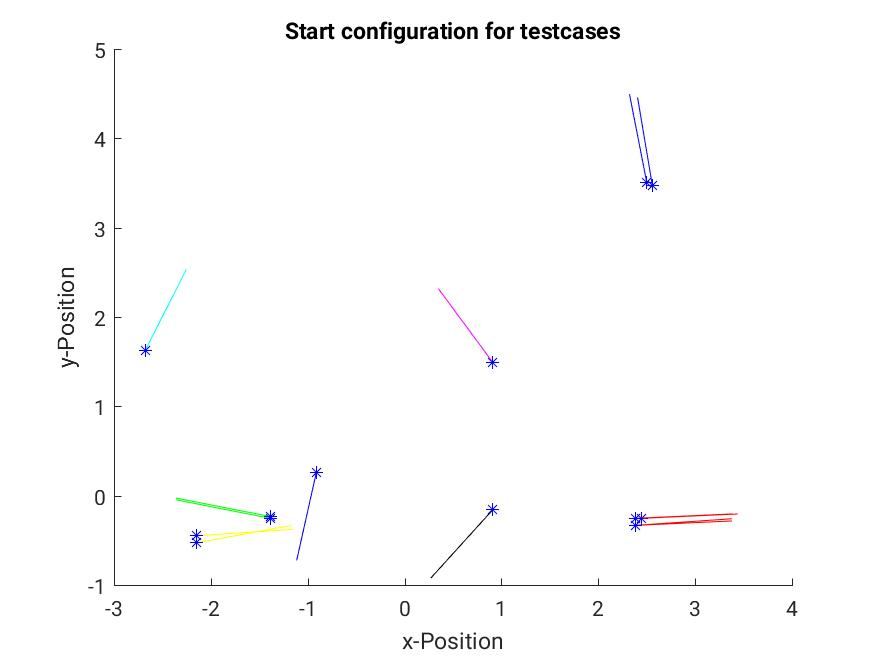
\includegraphics[width=.45\textwidth]{plain-tcs.jpg}
	}
	\caption{Migrationsfreie Evolution mit 5000 Generationen}
\end{figure}
}

\frame{
\frametitle{Migrationsfreier Durchlauf}
\begin{figure}
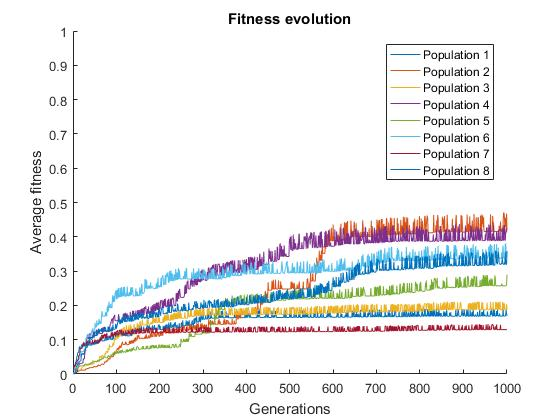
\includegraphics[width=.45\textwidth]{mig_free_fit.jpg}
\caption{Migrationsfreie Evolution mit 1000 Generationen}
\end{figure}
}

\frame{
\frametitle{Ergebnis: Schlechte Konfigurationen}
Hohe Migrationsraten werfen die Populationen weit zurück.\\
\begin{figure}
\centering
	\subfigure[Hohe Migrationsrate\label{fig:high_migrate}]{
		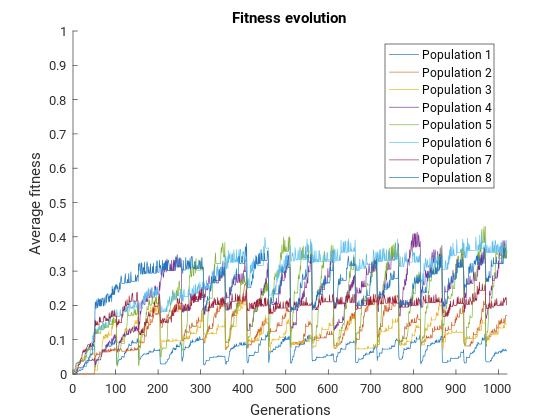
\includegraphics[width=.4\textwidth]{high_migrate.jpg}
	 }
	 \subfigure[Mittlere Migrationsrate\label{fig:mid_migrate}]{
		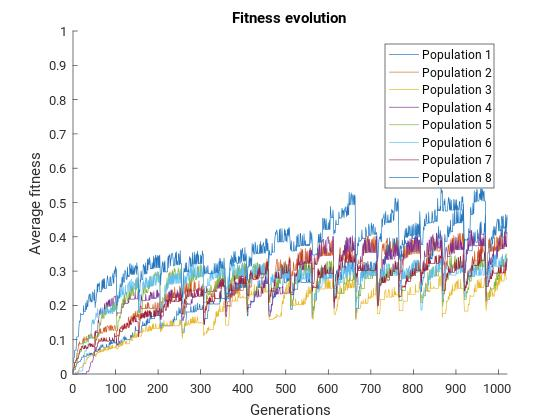
\includegraphics[width=.4\textwidth]{mid_migrate.jpg}
	 }
	 \caption{Migration alle 50 Generationen}
\end{figure}
}

\frame{
\frametitle{Ergebnis: Schlechte Konfigurationen}
Kleine Migrationszyklen führen zu nicht differenzierbaren Ergebnissen.\\
\begin{figure}
\centering
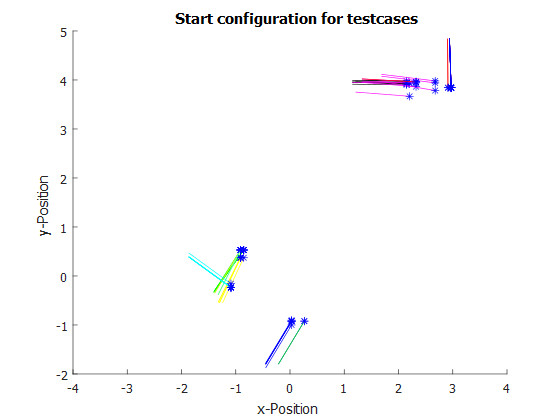
\includegraphics[width = .45\textwidth]{low_cs_tcs.jpg}
\caption{Migration jede Generation. Testfälle}
\end{figure}
}

\frame{
\frametitle{Ergebnis: Gute Konfigurationen}
Kleine Migrationszyklen führen zu schneller Gesamtkonvergenz.\\
\begin{figure}
\centering
\subfigure[Kleine Migrationszyklen\label{fig:small_cycles}]{
	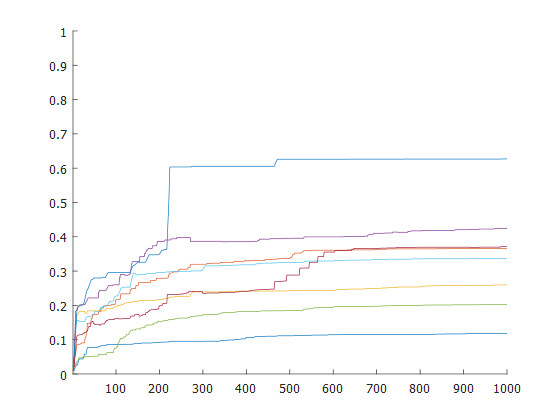
\includegraphics[width=.4\textwidth]{policy-ring_migRate-1_cycleSize-1-fit_alt.jpg}
}
\subfigure[Große Migrationszyklen\label{fig:big_cycles}]{
	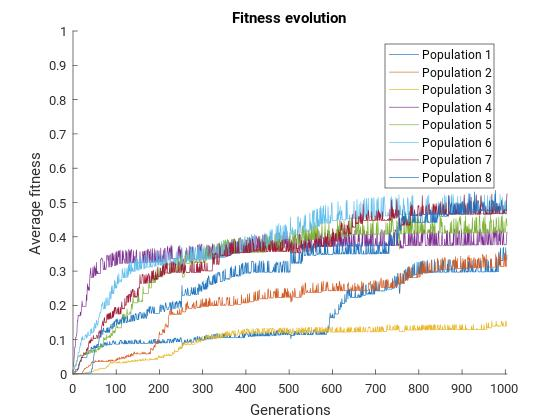
\includegraphics[width=.4\textwidth]{policy-ring_migRate-1_cycleSize-250-fit.jpg}
}
\caption{Fitness unterschiedlicher Migrationszyklus-Längen}
\end{figure}
}

\frame{
\frametitle{Ergebnis: Policy}
Neighbour konvergiert aufgrund semantischer Partnerwahl am schnellsten
\begin{figure}
\centering
\subfigure[Ring Policy\label{fig:pol_open}]{
	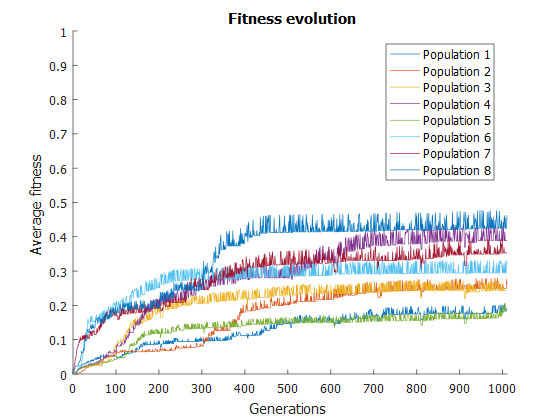
\includegraphics[width=.4\textwidth]{mig_ring_cs100_mr1.jpg}
}
\subfigure[Neighbour Policy\label{fig:pol_neigh}]{
	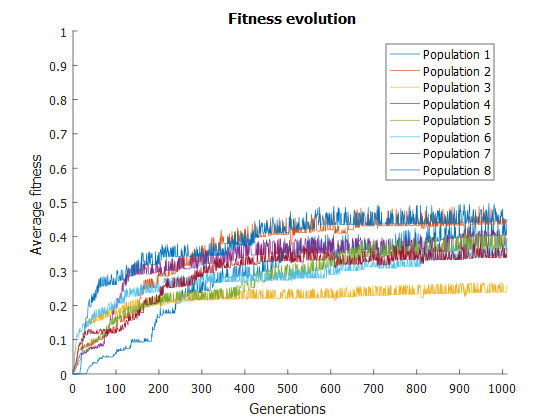
\includegraphics[width=.4\textwidth]{mig_neigh_cs100_mr1.jpg}
}
\caption{Fitness unterschiedlicher Migration Policies}
\end{figure}
}

\frame{
\frametitle{Ergebnis: Gute Konfigurationen}
Große Migrationzyklen führen zu differenzierbaren Ergebnissen.\\
\begin{figure}
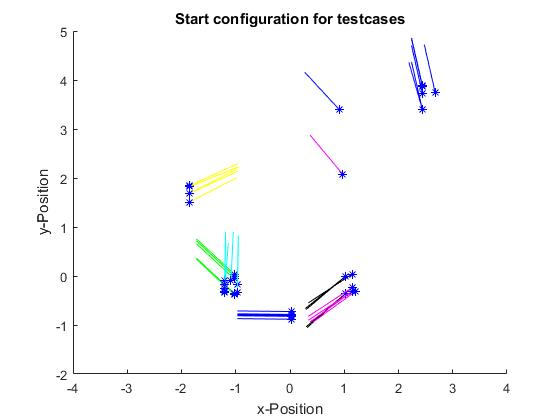
\includegraphics[width=.45\textwidth]{high_cs_tcs.jpg}
\caption{Migration mit großen Migrationszyklen. Testfälle}
\end{figure}
}

\frame{
\frametitle{Ergebnis: Zusammenfassung}
Im Vergleich:
\begin{enumerate}
	\item Konfigurationen untereinander
	\item Multi- vs Single-Population Genetic Algorithm
\end{enumerate}
}

\frame{
\frametitle{Ergebnis: Zusammenfassung}
\begin{enumerate}
	\item 
	Mittlere bis Kleine Migrationszyklen bei kleiner Migrationsrate führt zu den besten Durchläufen.
	\begin{itemize}
		\item Kleine Migrationsraten $>$ Große Migrationsraten
		\item Kleine Migrationszyklen sind schneller als große
		\item Große Migrationszyklen sind 'besser' als kleine
	\end{itemize}
	\item Multi Population GA im Allgemeinen besser als Single Population GA
	\begin{itemize}
		\item Ergebnisse der MPGA Populationen sind sich populationsübergreifend ähnlicher als bei normalen GA
		\item Konvergenz von MPGAs erfolgt schneller als bei normalen GA
	\end{itemize}
\end{enumerate}
}

\end{document}